\nsection{Problem 2 - (Sequential Monte Carlo)}
In spatial statistics there are many different approaches
for modelling continuity of discrete properties in a region. One method which is popular due
to the intuitive interpretation is the truncated Gaussian model. In this model one generates a
Gaussian random field in $\mathbb{R}^d$ and divide the value set into intervals to define the classes. When applying the model, it is challenging to get the parameters of the model right. One way to get the parameters correct is to estimate them from training data. In this case we have a map of discrete values and want to derive the properties of the underlying Gaussian random field. This is the situation we will investigate below. We will however restrict focus to 1D in this exercise.

The model is given as:
\begin{align}
    x_1 &\sim \mathcal{N}(0,1) \\[5pt] 
    x_t &= ax_{t-1} + \lambda + \varepsilon_t, \quad t = 2, 3, \ldots \\[5pt]
    \varepsilon_t &\sim \mathcal{N}(0, \sigma^2), \quad t = 2,3, \ldots \\[5pt] 
    y_t &= 
    \begin{cases}
        1  &\text{ if } x < -0.5 \\[5pt]
        2  &\text{ if } -0.5 \leq x < 0.5 \\[5pt]
        3  &\text{ if } x \geq 0.5 
    \end{cases}
    ,\quad t = 2,3, \ldots
\end{align}
\nssection{a.)}
\emph{Design a sequential Monte Carlo algorithm for inference about $p(x_t | \boldsymbol{y}_{1:t}), \ t= 1, 2, \ldots, n$, assuming that $(a, \lambda, \sigma^2) = (0.85, 0, 0.5^2)$. Display plot of $\mathbb{E}(x_t | \boldsymbol{y}_{1:t})$ and $\text{Var}(x_t | \boldsymbol{y}_{1:t})$. Give arguments for the choices you make in the construction.} \spaze
\textbf{Solution:} \spaze
The implementation can be found in Appendix (\ref{appendix:b}), from code listings (\ref{lst:MC_2a}), and produces the following plots: 
\begin{figure}[H]
    \centering
    \begin{subfigure}[b]{0.45\textwidth}
        \centering
        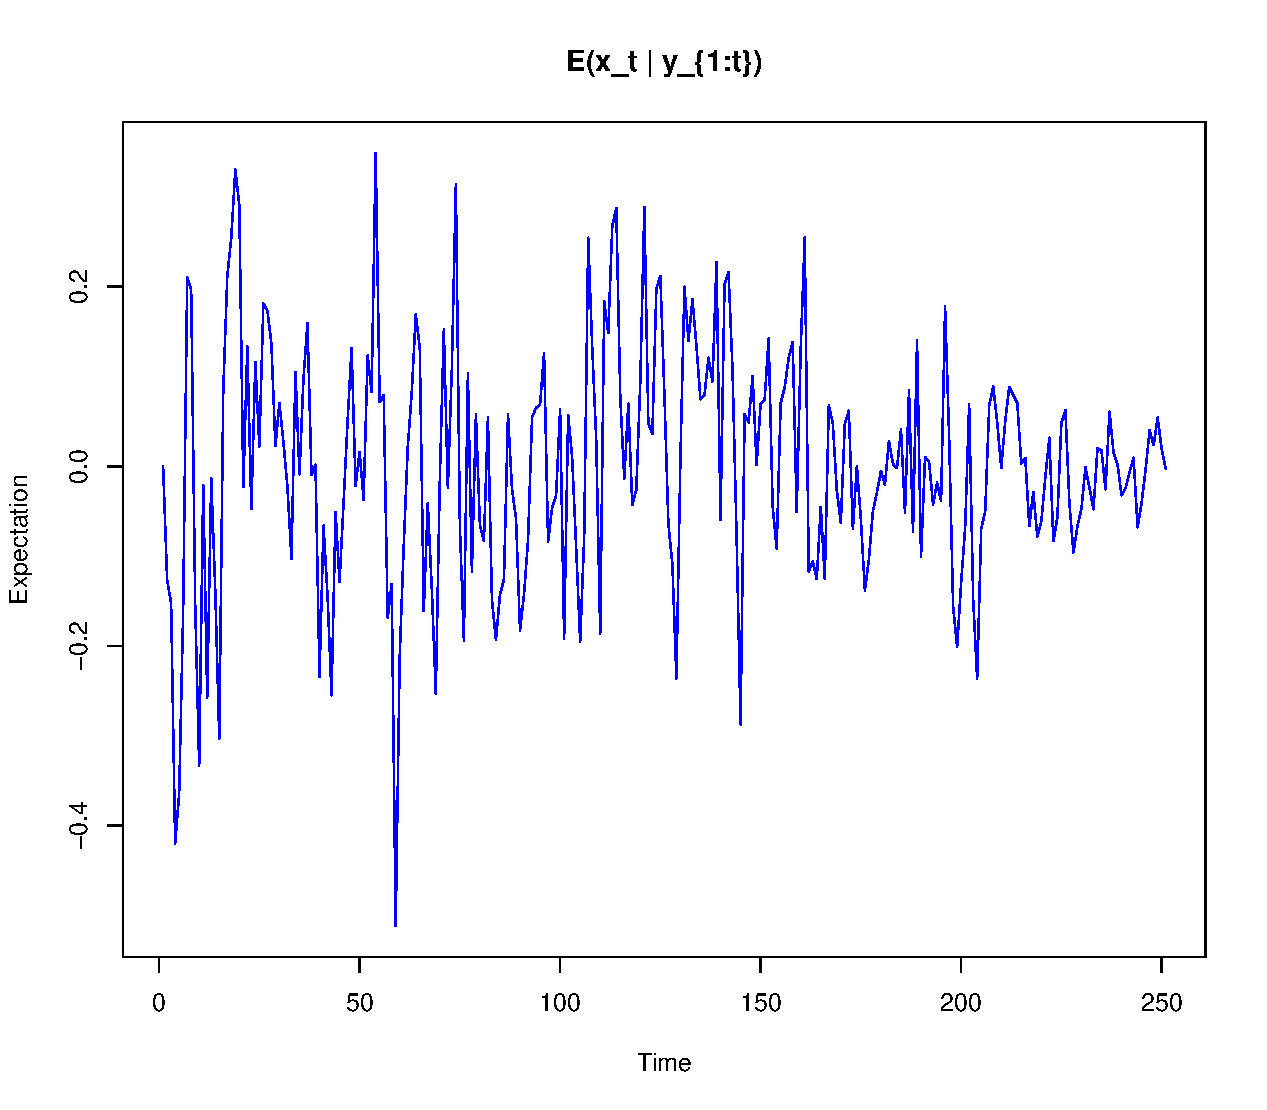
\includegraphics[width=\textwidth]{Images/Exercise_2_Figures/SMC_2a.pdf} 
        \caption{$\mathbb{E}(x_t | \boldsymbol{y}_{1:t})$}
        \label{fig:sub1}
    \end{subfigure}
    \hfill
    \begin{subfigure}[b]{0.45\textwidth}
        \centering
        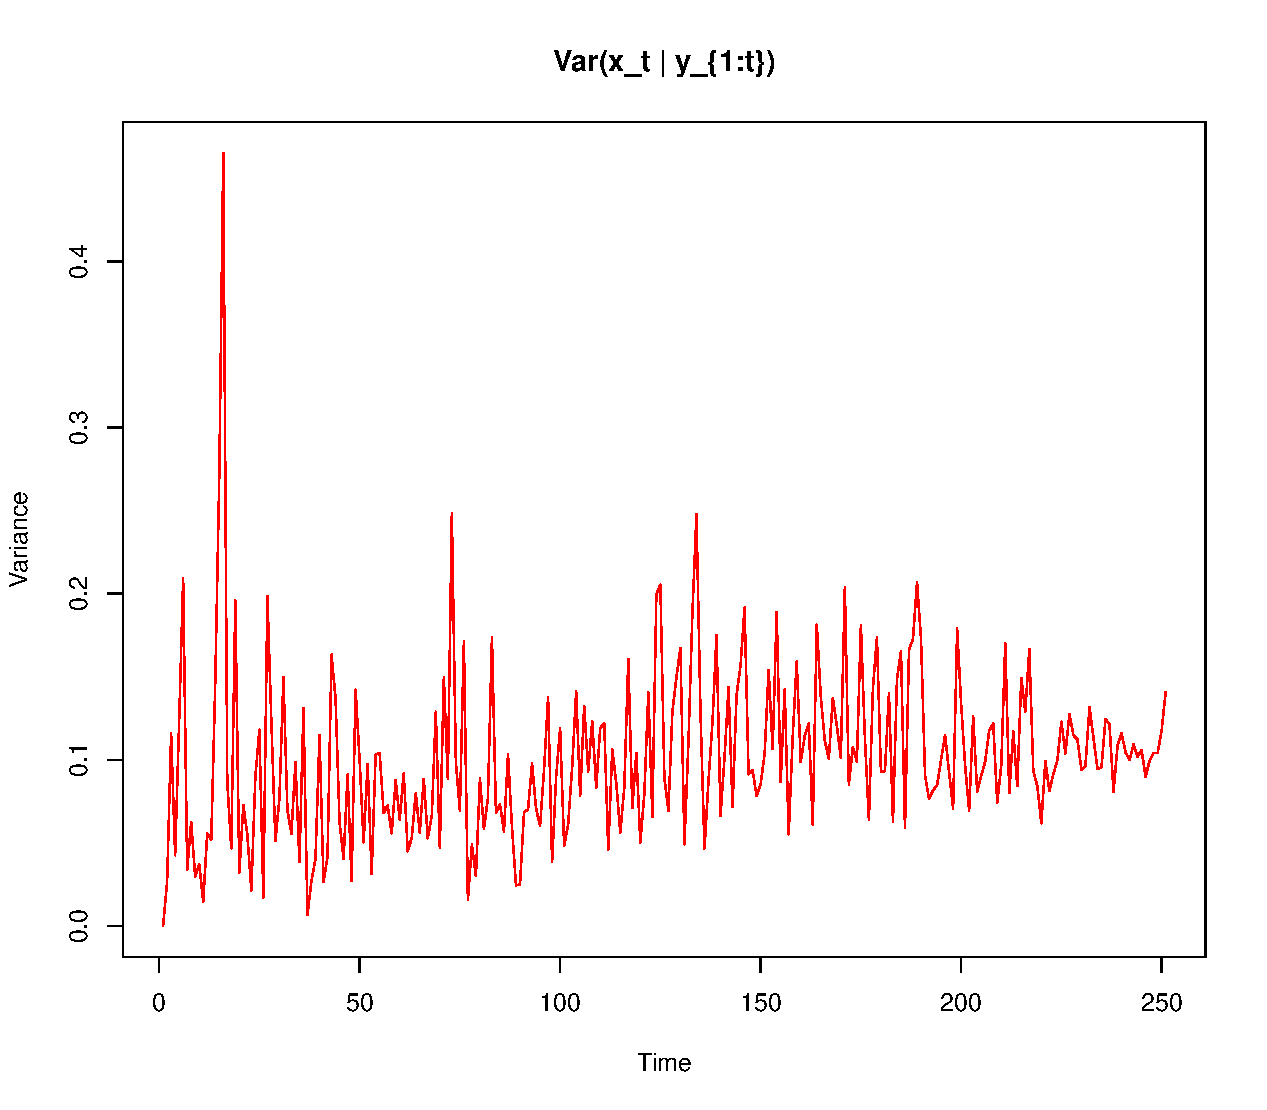
\includegraphics[width=\textwidth]{Images/Exercise_2_Figures/SMC_2b.pdf} 
        \caption{$\text{Var}(x_t | \boldsymbol{y}_{1:t})$}
        \label{fig:sub2}
    \end{subfigure}
    \caption{Sequential Monte Carlo Simulation estimation of $\mathbb{E}(x_t | \boldsymbol{y}_{1:t})$ and $\text{Var}(x_t | \boldsymbol{y}_{1:t})$}
    \label{fig:overall}
\end{figure}
In construction of the sequential Monte Carlo (SMC) algorithm, the choice of 1000 particles was chosen to balance out the ratio of computational effort and accuracy of estimation. The particles are initialized with zero values for simplicity, and weights are initialized with equal weights. The resampling is applied to address potential particle degeneracy, such that it maintains diverse candidate solutions and make that particles with higher weights are retained for the next iteration. Here, I have used simple multinomial resampling with replacement. Lastly, importance weights are calculated based on the likelihood of observing the data given the particles' states.
\nssection{b.)}
\emph{We will use sequential Monte Carlo to perform online learning algorithm for the parameter .
For simplicity we will assume that $(\lambda, \sigma^2) = (0, 0.5^2)$ is fixed and known.} 

\emph{Consider a prior model for $a$ which is uniform on the interval $[0, 1]$. Design and
implement a sequential Monte Carlo algorithm for inference about $a$, i.e.
estimate $p(a | \boldsymbol{y}_{1:251})$. Use a static approach, i.e. sample $a$ initially from the prior distribution, and update it by weighting/resampling throughout the simulation. Why is this approach in general not recommended? Comment on your results, are these
acceptable?}\spaze
\textbf{Solution:} \spaze
The implementation can be found in Appendix (\ref{appendix:b}), from code listings (\ref{lst:MC_2b}), and produces the following output: 
\begin{align*}
     p(a | \boldsymbol{y}_{1:251}) = 0.41077276906278
\end{align*}